\chapter{Introdução}

A introdução eu devo escrever por último, deve conter a importancia do projeto, devo descrever o problema e a solução: "existe um problema e foi resolvido assim". O final da introdução deve descrever a estrutura dos capitulos dando uma pincelada rapida em cada um.

\chapter{Conceitos}
\section{Arquitetura de Software}
\section{Atributos de Modularidade}
\subsection{Acoplamento}
\subsection{Coesão}

\chapter{Implementação do Extrator}

Neste capítulo deve documentar o que fiz e como fiz, as dificuldades encontradas no processo, etc...
\section{egypt}
\section{Doxygen (e a sua API)}
\section{Implementação do Extrator usando a API do Doxygen}

\chapter{Avaliação}
\section{Procedimento}
\section{Resultados}

Nos resultados eu posso comparar o que consegui com a nova ferramenta comparado ao modo antigo do egypt extrair informacoes.

\begin{figure}[h]
\center
\subfigure[ristretto-0.0.1-doxyparse][Egypt::Extrator::Doxyparse]{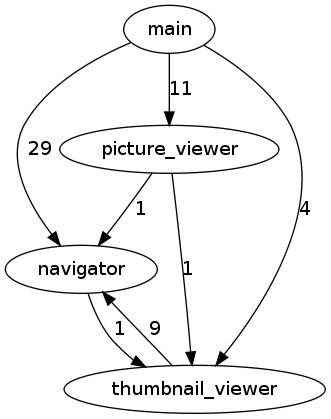
\includegraphics[scale=0.5]{imagens/ristretto-0_0_1-doxyparse}}
\qquad
\subfigure[ristretto-0.0.1-gcc][Egypt::Extrator::GCC]{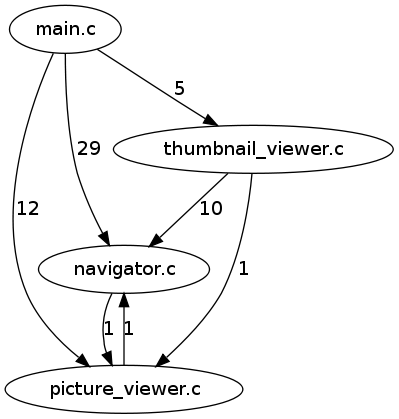
\includegraphics[scale=0.5]{imagens/ristretto-0_0_1-gcc}}
\caption{gráfico de chamada entre módulos do {\bf Ristretto 0.0.1} gerado pelo Egypt}
\end{figure}

\begin{figure}[h]
\center
\subfigure[ristretto-0.0.11-doxyparse][Egypt::Extrator::Doxyparse]{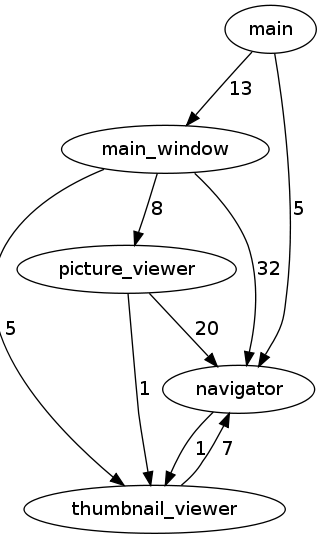
\includegraphics[scale=0.5]{imagens/ristretto-0_0_11-doxyparse}}
\qquad
\subfigure[ristretto-0.0.11-gcc][Egypt::Extrator::GCC]{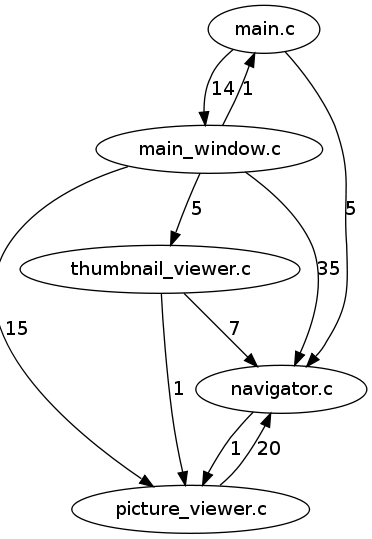
\includegraphics[scale=0.5]{imagens/ristretto-0_0_11-gcc}}
\caption{gráfico de chamada entre módulos do {\bf Ristretto 0.0.11} gerado pelo Egypt}
\end{figure}

\begin{figure}[h]
\center
\subfigure[ristretto-0.0.21-doxyparse][Egypt::Extrator::Doxyparse]{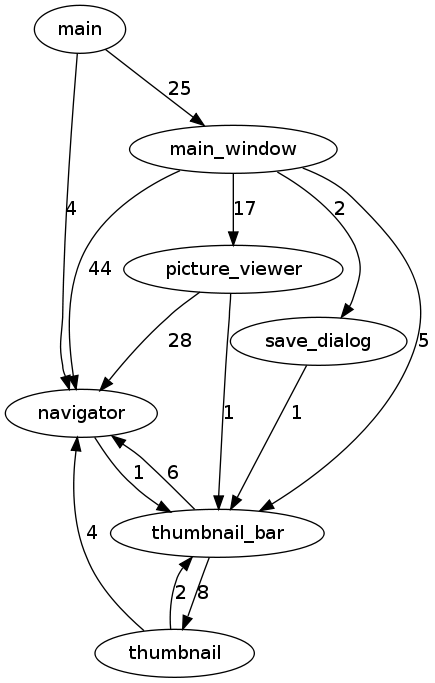
\includegraphics[scale=0.5]{imagens/ristretto-0_0_21-doxyparse}}
\qquad
\subfigure[ristretto-0.0.21-gcc][Egypt::Extrator::GCC]{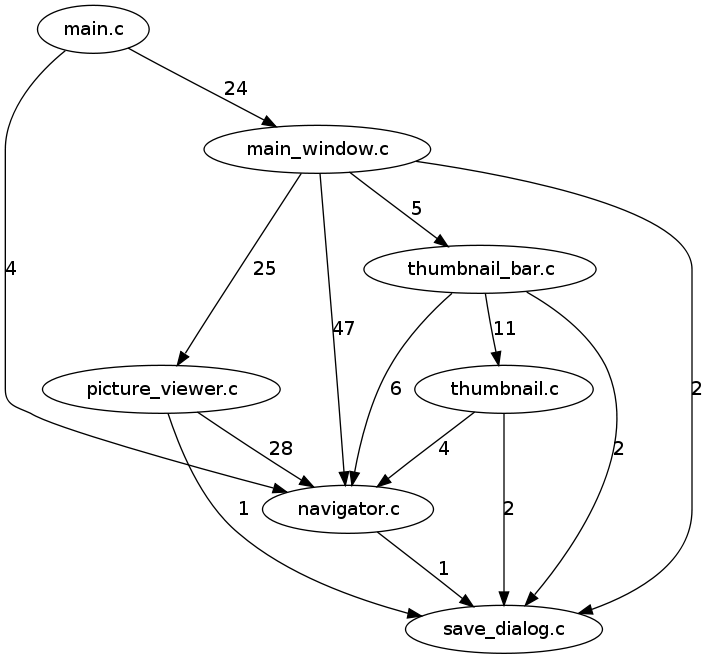
\includegraphics[scale=0.5]{imagens/ristretto-0_0_21-gcc}}
\caption{gráfico de chamada entre módulos do {\bf Ristretto 0.0.21} gerado pelo Egypt}
\end{figure}

\section{Discussão}

\chapter{Conclusão}

A conclusão eu devo escrever por último, deve conter algo assim: "Este trabalho tinha objetivo tal e atingiu tal objetivo". Deve ter referencia de como foi feito e se os resultados foram bons, medios, satisfatorios, ruins, etc. E ao final deve ter trabalhos futuros que eu tenha interesse ou não de fazer.
